\documentclass{article}
\usepackage{geometry}
\geometry{a4paper, scale=0.8}

\usepackage[utf8]{inputenc}
\usepackage{ctex}
\usepackage{assignpkg}
\usepackage{amsmath}
\usepackage{amssymb}
\studentIds{202XX80XXXXXXXX}{}
\studentNames{XXX}{}

\assignmentNumber{4}

\date{\today}

\begin{document}

\makecover
\subsection*{1. 列举几种常见的半监督学习方法。比较有监督学习、无监督学习、半监督学习、主动 学习以及强化学习的异同;}
\begin{itemize}
\item[(1)]
常见的半监督学习方法:

半监督学习可分为半监督分类问题和半监督聚类问题

半监督分类问题的方法可以可分为如下几大类:启发式方法、生成式方法、半监督SVM、直推式SVM(TSVM)、图半监督学习和基于分歧的方法。其中最后一个为基于多分类器的问题,前面的方法为基于单分类器的问题。

半监督聚类问题的方法有约束k均值算法和约束种子k均值算法。
\item[(b)]
各种学习的不同之处:

监督学习:给定输入和输出,估计输入和输出之间的函数;常见的学习问题如分类和回归

无监督学习:仅给定输入,没有对应的输出以及环境反馈等;常见的学习问题如密度估计、聚类

半监督学习:介于监督学习和无监督学习之间,给定少量标记样本和大量无标记样本进行函数估计

强化学习:试图让机器学会如何进行自动决策,特点:没有监督信息,仅有环境反馈的奖励信号;环境的反馈具有滞后性,不能立即得到;时间(序列)是一个重要因素,数据不具有独立同分布特性;智能体的当前动作会影响后续获取的数据。

主动学习:首先利用少量标记样本训练得到一个模型,然后从未训练样本中选择一些标记样本向用户询问其标记,将这些新得知其标记的样本加入训练集重新得到一个模型;多次重复上述过程。主动学习引入了额外的专家知识,通过外界的交互来将部分未标记的样本转变为有标记的样本。
\item[(c)]
相同之处:

除了无监督学习和强化学习之外,其他学习都涉及到样本的标记。

在有监督学习和半监督学习中,都存在连续假设,即假设邻近点的标签应该一致。但不同之处在于前者倾向于得到简单的决策边界,后者倾向于在低密度数据点区域构造决策边界。

半监督学习和无监督学习都涉及到与聚类相关的问题。

半监督学习和有监督学习都涉及到分类和回归的问题。

\end{itemize}

\subsection*{2. 试给出协同训练的方法步骤;}
协同训练的基本步骤:
\begin{itemize}
\item[1]
首先,在每个视图上基于有标记样本分别训练一个分类器;
\item[2]
然后,让每个分类器分别去挑选自己“最有把握的”未标记样本赋予伪标记,并将伪标记样本提供给另一个分类器作为新增的有标记样本用于训练更新;
\item[3]
不断迭代上述步骤(“互相学习,共同进步”),直到两个分类器都不再发生变化,或达到预定的迭代轮数为止
\end{itemize}

\subsection*{程序设计题}
源代码文件见code文件夹。此项目包含两个文件,rl.py和plotLearningCurve.py。
rl.py文件中包含了一个learn()函数,通过设置method参数值可选择学习的方法是Qlearning还是Sarsa。

下面是关于learn函数的更详细的描述:
该函数通过传入的学习率、折扣因子、学习方法等参数对冰湖游戏进行强化学习。
\subsubsection*{learn(learning\_rate = 0.8, gamma = 0.95, method=Qlearning)}
\begin{itemize}
\item parameters: learning\_rate, gamma, method
	\begin{itemize}
		\item[-] 
		learning\_rate: 学习率
		\item[-] 
		gamma: 折扣因子
		\item[-] 
		method: 值为常量Qlearing=1时,将使用Qlearning方法进行强化学习,否则使用Sarsa方法
	\end{itemize}
\item returns: learning\_data

leaning\_data是一个total\_episodes*3的数组,其中total\_episodes是一次学习的次数的总次数,三个维度分别记录了每次游戏结束时所走的步数,获得的奖励值,以及到当前累计的奖励值。

\end{itemize}

也就是说rl.py文件实现了Qlearning和Sarsa算法,而plotLearningCurve.py文件则是用来通过设置不同的参数值来分析这些参数对学习过程的影响的。

\subsubsection*{分析不同学习率和折扣因子下Sarsa算法的表现}
\begin{itemize}
\item 
不同折扣因子下Sarsa算法的表现,如图\ref{fig:1}
\begin{figure}[htbp]
	\centering
	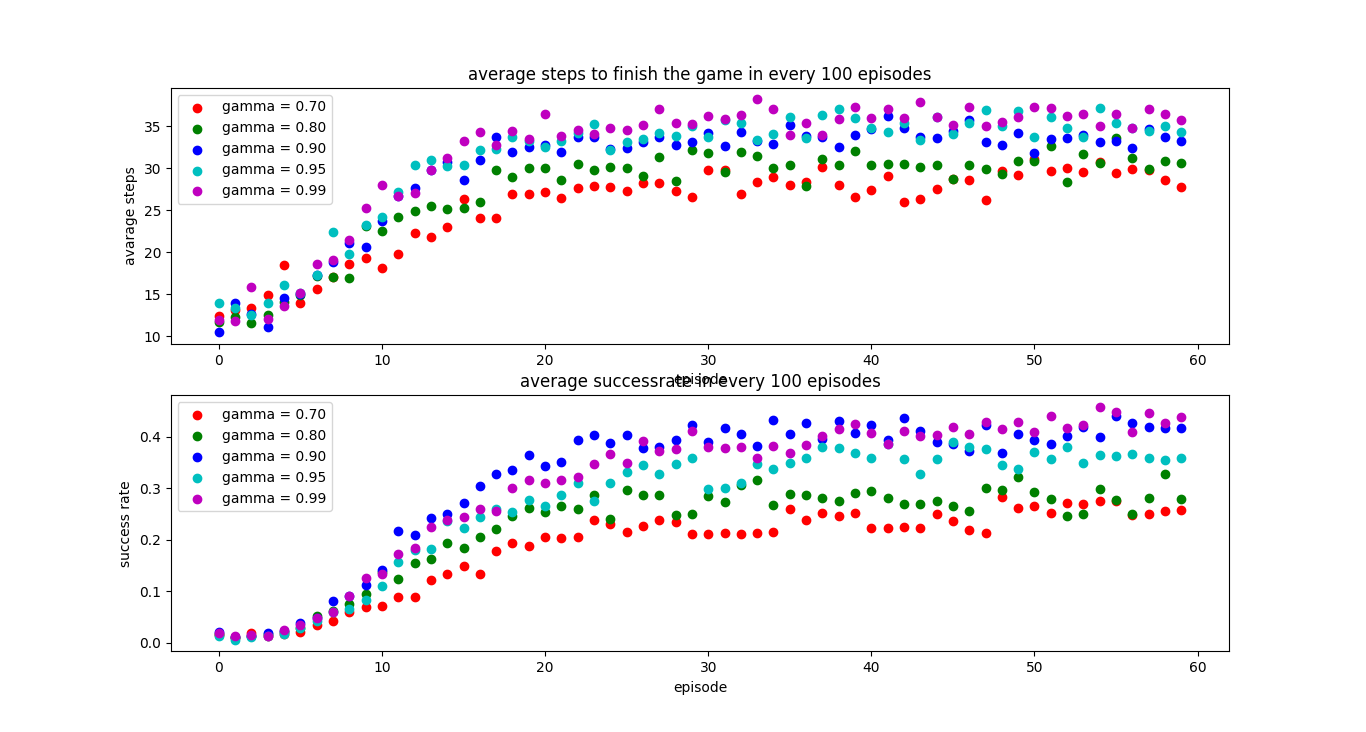
\includegraphics[scale=0.5]{Img/Sarsa_gamma.png}
	\caption{不同折扣因子下Sarsa算法的表现}\label{fig:1}
\end{figure}

其中折扣因子的大小我选择的是0.7,0.8,0.9,0.95,0.99。

我用两个因素来评价算法的性能,算法成功需要的步数和算法的成功率。

按照算法成功需要的步数来看,几个参数下算法的性能排序如下:0.7>0.8>0.9>0.95>0.99

按照算法成功率来看,这几个参数下算法的性能排序如下:0.99>0.9>0.95>0.8>0.7

可以看出,照这两个标准,将得到截然相反的结果。这说明,折扣因子越大,算法越谨慎,越不敢往前走,所以成功所需花费的步数愈多。

而对于成功率而言,则是折扣因子越大,其成功率越高,但是在0.9-0.99这个区间还需要更多的数据来观察其规律,由于时间关系,就没有进一步探索其关系。

\item
不同学习率下Sarsa算法的表现,如图\ref{fig:2}
\begin{figure}[htbp]
	\centering
	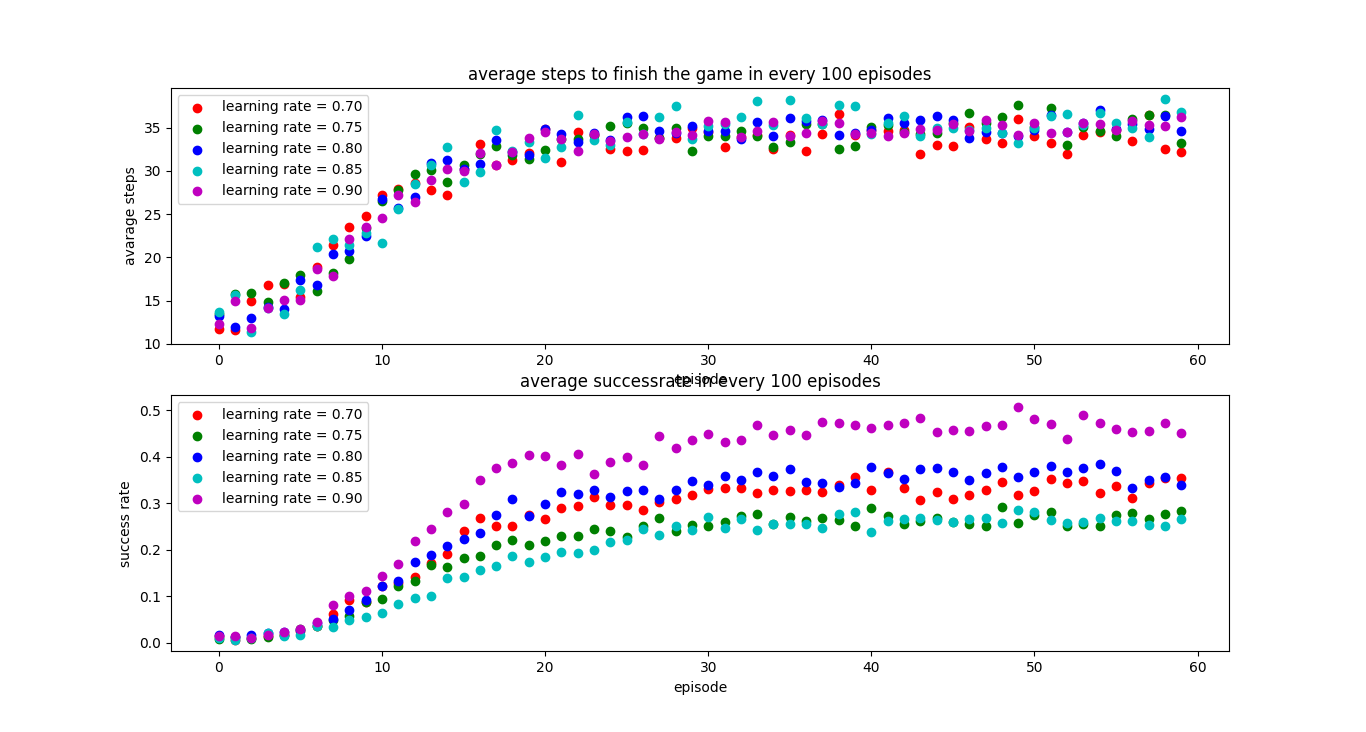
\includegraphics[scale=0.5]{Img/Sarsa_lr.png}
	\caption{不同学习率下Sarsa算法的表现}\label{fig:2}
\end{figure}

其中学习率的大小我选择的是0.7,0.75,0.8,0.85,0.9。

按照算法成功需要的步数来看,几个参数下算法的性能有如下规律:
\begin{itemize}
\item 学习率为0.7的所需的步数相对来说是最少的,它比较大胆
\item 学习率为0.9的发挥比较稳定,平均所需花的步数处于适中的水平。
\item 在步数波动上,按拨动从大到小的顺序依次大概是:0.7=0.75=0.85>0.8>0.9
\end{itemize}

按照算法成功率来看,这几个参数下算法的性能排序如下:0.9>0.8>0.7>0.75=0.85。

这个规律性不是很明显,但是看起来貌似是保留一位小数的更占优势。但趋势是越高的学习率,会有更高的成功率。
\end{itemize}
%\clearpage
\subsubsection*{分析不同学习率和折扣因子下Qlearning算法的表现}
\begin{itemize}
\item 
不同折扣因子下Qlearning算法的表现,如图\ref{fig:3}
\begin{figure}[htbp]
	\centering
	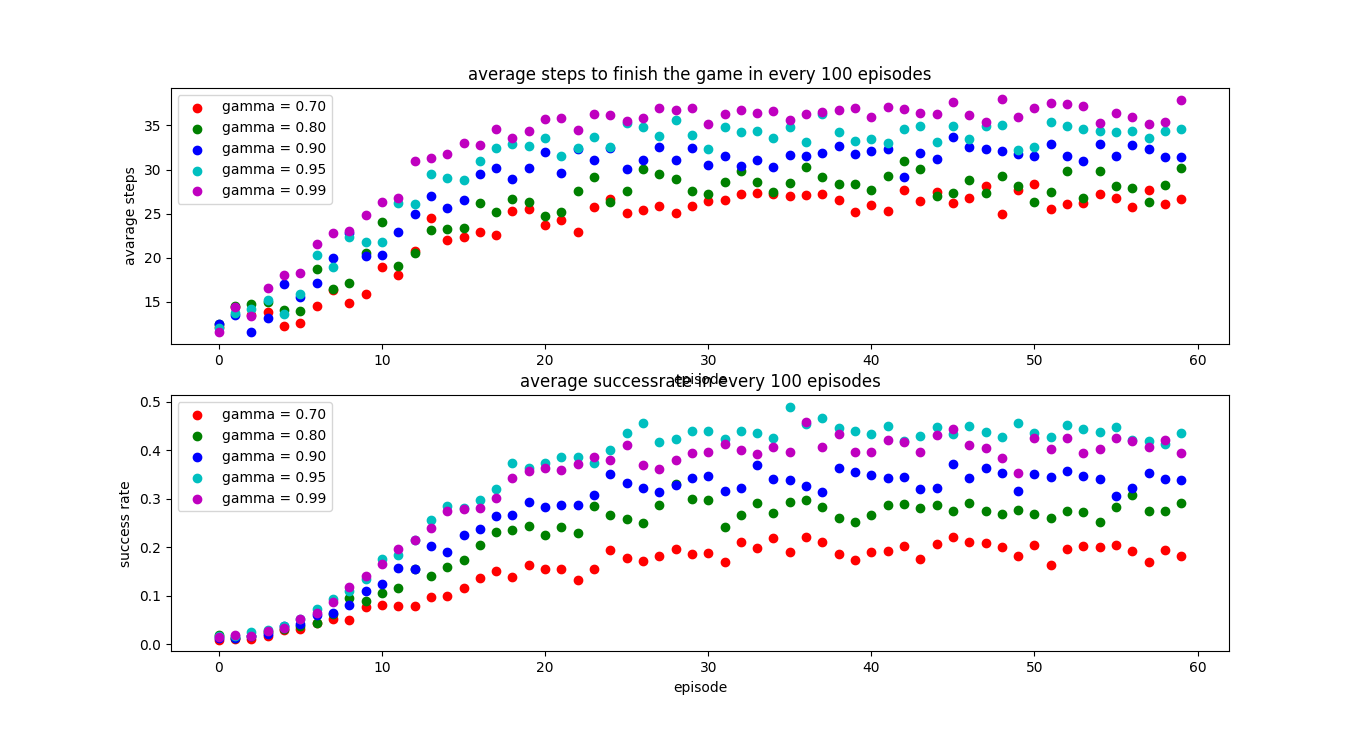
\includegraphics[scale=0.5]{Img/Qlearning_gamma.png}
	\caption{不同折扣因子下Qlearning算法的表现}\label{fig:3}
\end{figure}

按照步数评价性能:0.7>0.8>0.9>0.95>0.99

按照成功率评价性能:0.95>0.99>0.9>0.8>0.7

两者仍然符合前述规律

两个算法中,0.95都取得了最高的成功率,说明0.95对于这个问题是一个不错的折扣因子。

\item 
不同学习率下Qlearning算法的表现,如图\ref{fig:4}

按照步数的标准来评价,其实这几个学习率下他们的的性能表现是难以区分出好坏的。所以不多做评价。

按照成功率来看,0.7>0.9>0.75>0.85>0.8

似乎呈现着以0.8附近成功率低,0.8两侧的学习率递增的趋势,即 0.7>0.75>0.8, 0.9>0.85>0.8。
究竟多大的学习率(0.9一侧还是0.7一侧)更适合还需要进一步试验。

\clearpage
\begin{figure}[htbp]
	\centering
	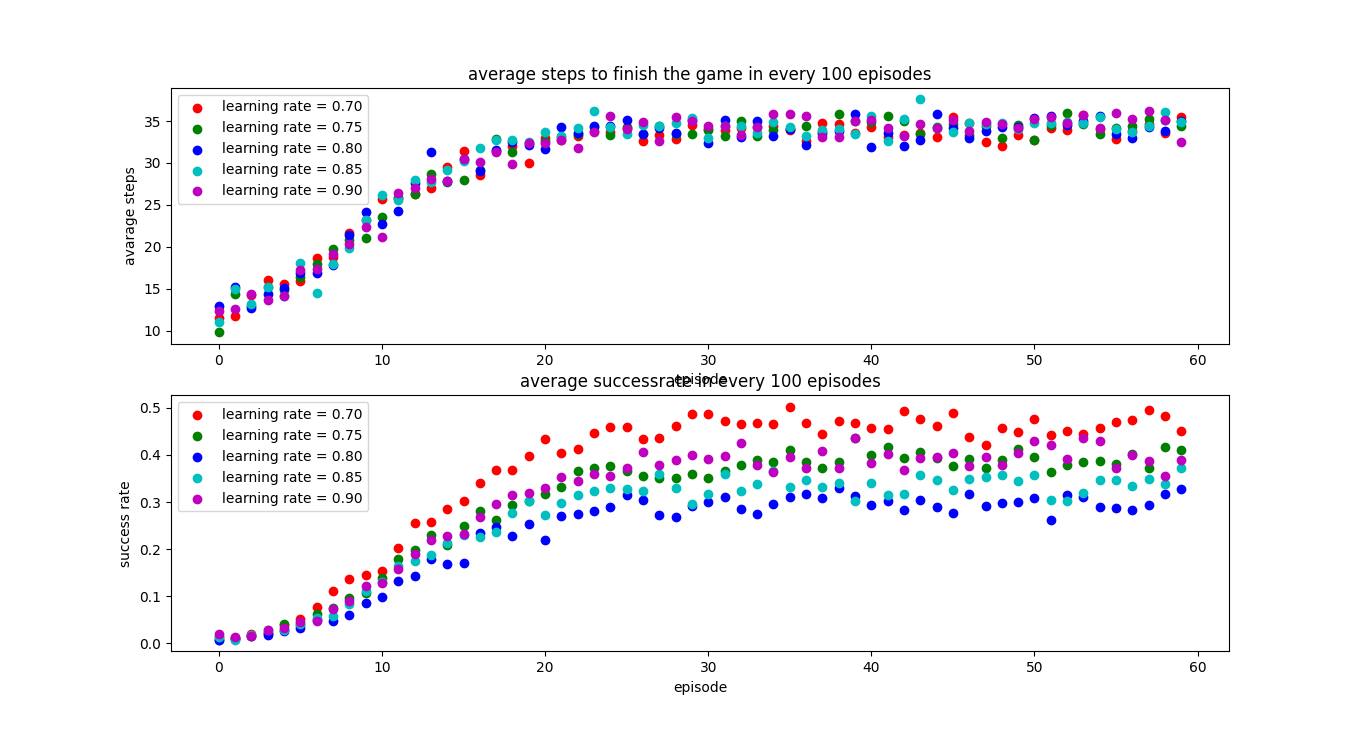
\includegraphics[scale=0.5]{Img/Qlearning_lr.png}
	\caption{不同学习率下Qlearning算法的表现}\label{fig:4}
\end{figure}
\end{itemize}

\subsubsection*{分析并实验对比上述两个算法的性能表现}
由于两个算法的最佳折扣因子都取0.95,我们通过选取三个不同的学习率(0.7, 0.8, 0.9)来对比两个算法的性能表现。

值得注意的是,0.7是Sarsa的最佳学习率,0.9是Qlearning的最佳学习率

得到结果如图\ref{fig:5},图\ref{fig:6},图\ref{fig:7}。可以看出

\begin{itemize}
\item 学习率为0.7时,Qlearning算法的性能高于Sarsa,而学习率为0.8,0.9时,Qlearning性能更低。
\item 考虑到0.9是Sarsa算法最偏好的学习率,并且Qlearning偏好于更低的学习率这两个事实倒也说得过去。
\item 我本以为两者在成功所需要的步数上,Sarsa算法的步数要多于Qlearning,但实际上,两者的步数伯仲之间。
\end{itemize}

\begin{figure}[htbp]
	\centering
	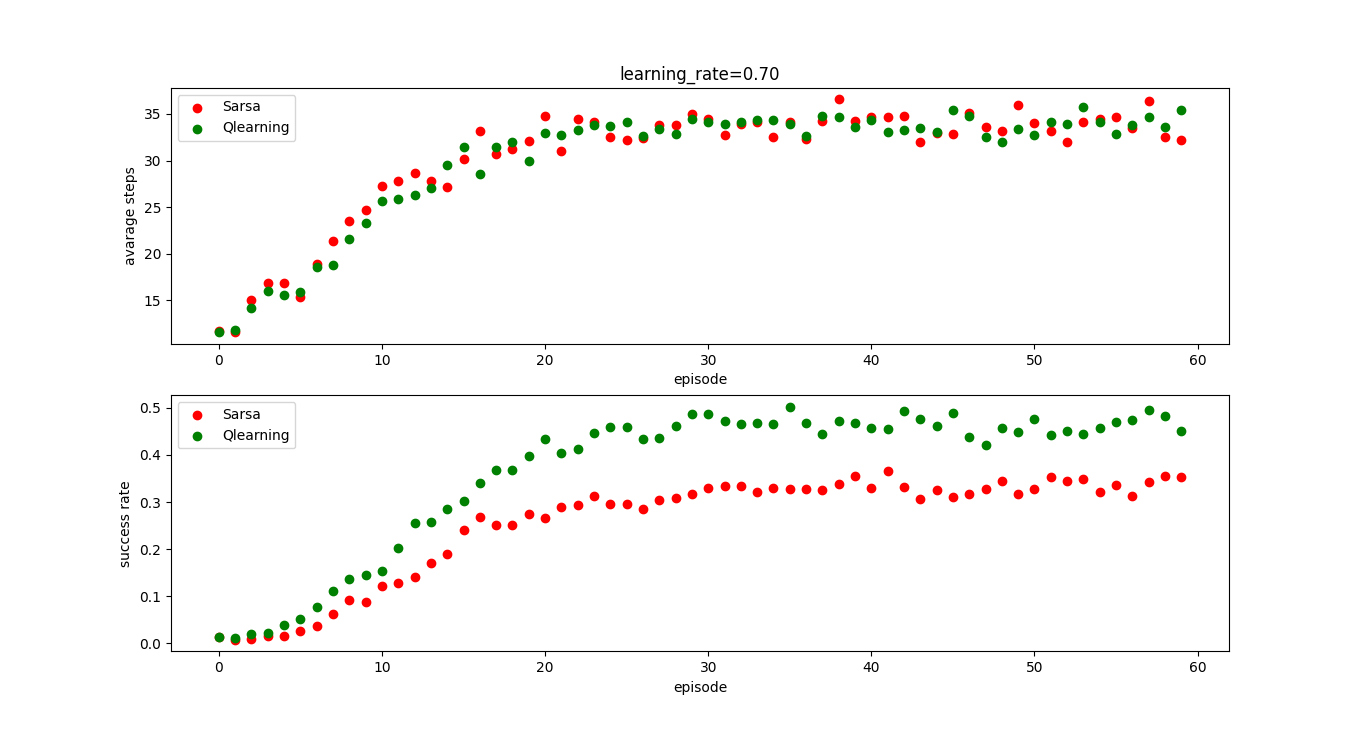
\includegraphics[scale=0.4]{Img/lr=0.7.png}
	\caption{lr=0.7}\label{fig:5}
	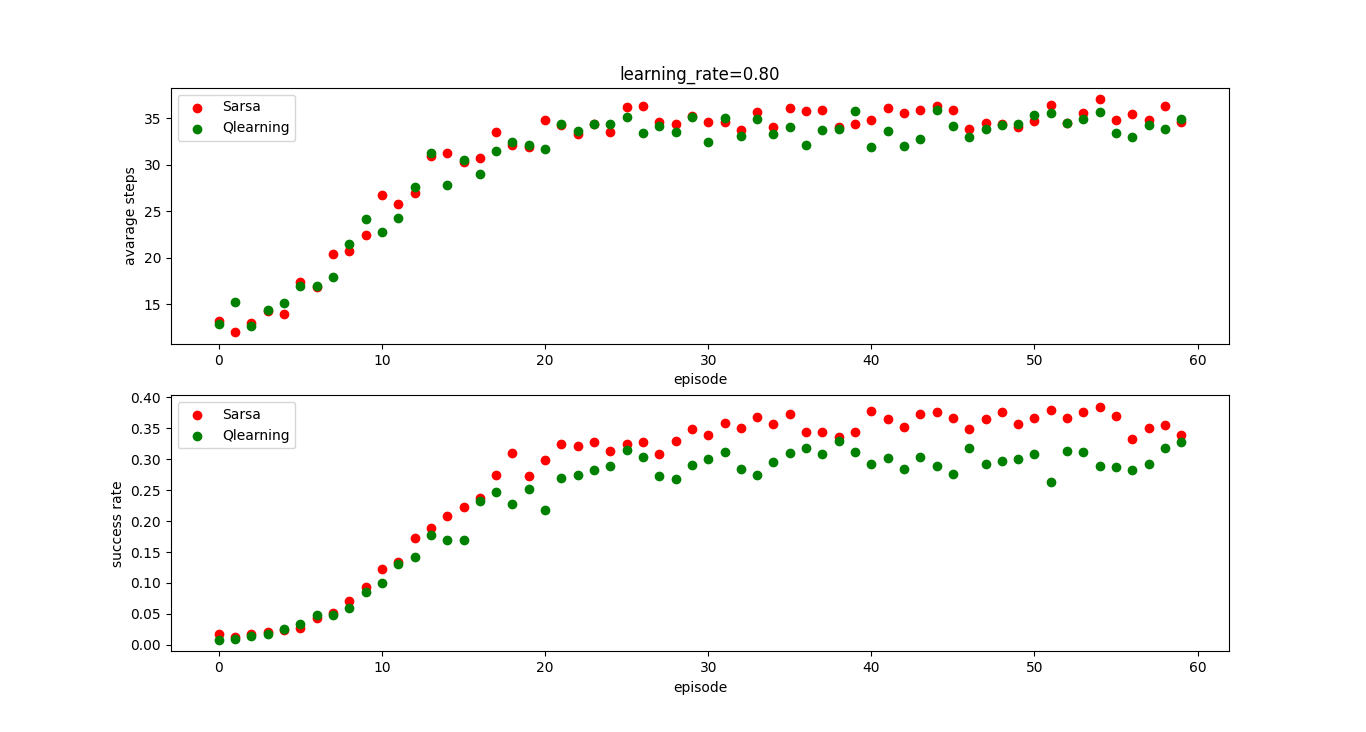
\includegraphics[scale=0.4]{Img/lr=0.8.png}
	\caption{lr=0.8}\label{fig:6}
	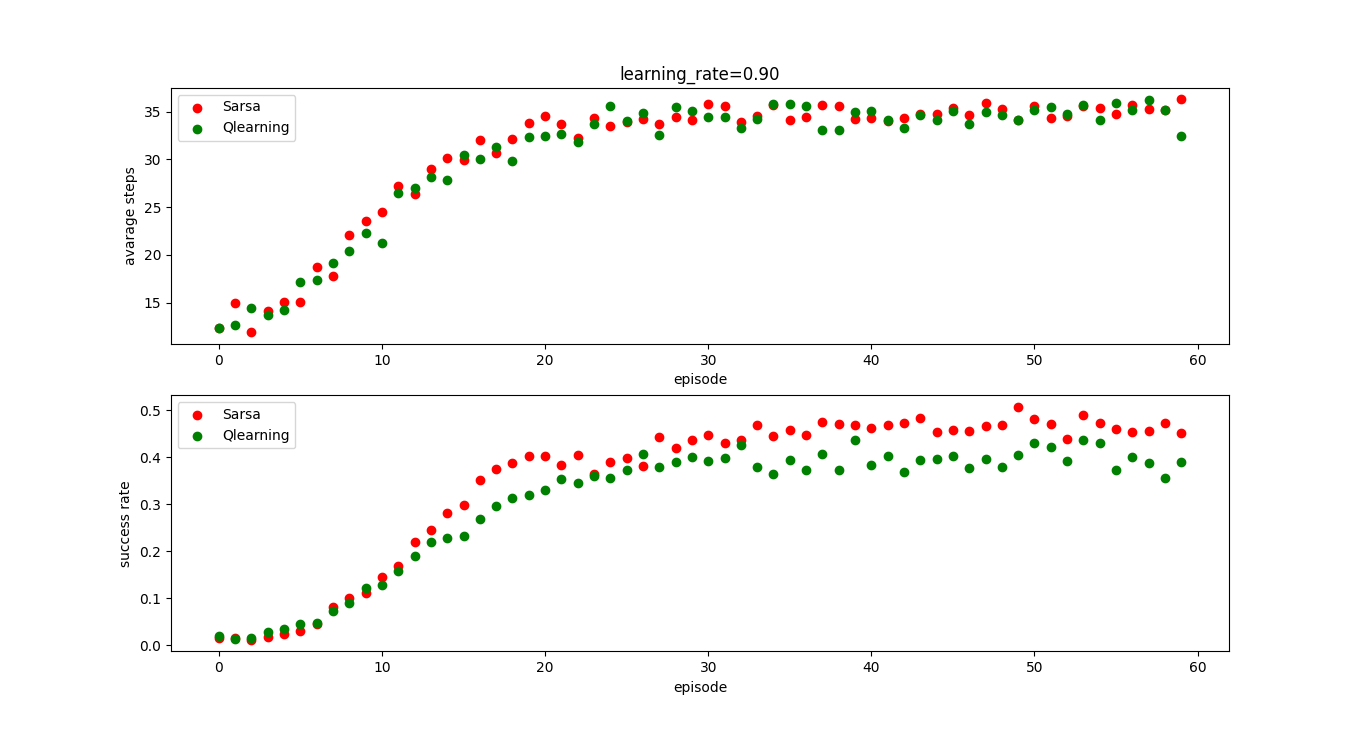
\includegraphics[scale=0.4]{Img/lr=0.9.png}
	\caption{lr=0.9}\label{fig:7}
\end{figure}


\end{document}
